\subsection{Cooling The Circuit Board:}

After removing the iron from the top of the circuit board with our fingers we make some pressure all around the circuit board just to make sure that the ink it's successfully transfer (Figure 3.3.0 ) then, we take the circuit board to a source of water and we hold the circuit board below it. An alternative approach is to immerse the board and paper in hot water for a few minutes ( up to 10 minutes like in Figure 3.3.1 and 3.3.2 ). \hfill \break

\begin{figure}[H]
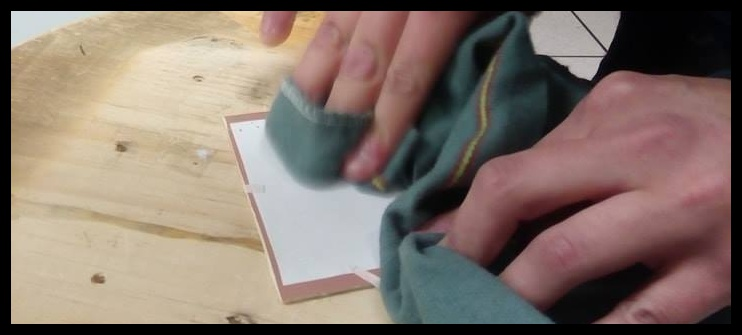
\includegraphics[height = 6cm, width = 16.5cm]{1f.jpg}
\centering \linebreak \linebreak {\small Figure 3.3.0: Pressing the circuit board to make sure that the ink it's successfully transferred.}
\end{figure}

\begin{figure}[H]
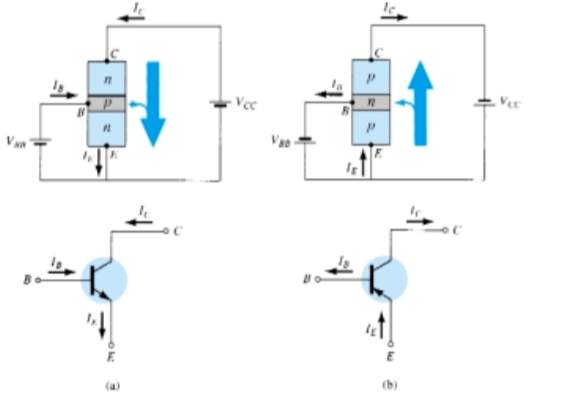
\includegraphics[height = 6cm, width = 16.5cm]{5.png}
\centering \linebreak \linebreak {\small Figure 3.3.1: Immersing the circuit in water.}
\end{figure}

\begin{figure}[H]
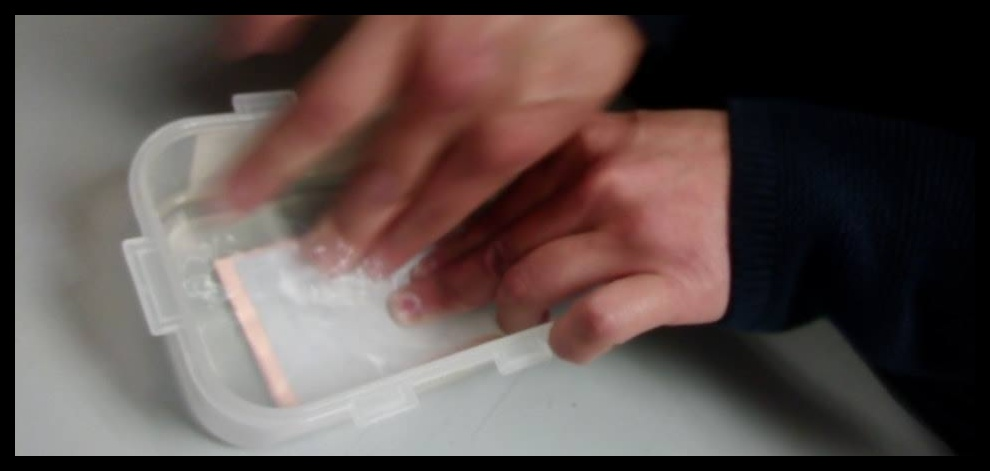
\includegraphics[height = 6cm, width = 16.5cm]{1g.jpg}
\centering \linebreak \linebreak {\small Figure 3.3.2: Immersing the circuit in water ( real ).}
\end{figure} \hfill \break

Slowly we start to take off the paper and soon all of the paper should come off. Finally, we have a copper board with our PCB pads and signal lines traced out in black toner like Figure 3.3.3 \hfill \break

\begin{figure}[H]
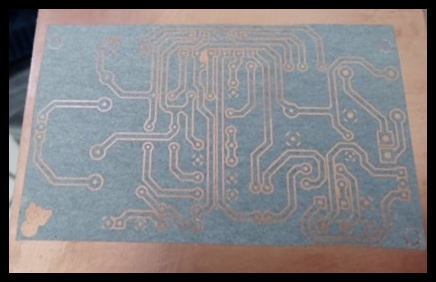
\includegraphics[height = 8cm, width = 16.5cm]{2b.jpg}
\centering \linebreak \linebreak {\small Figure 3.3.3: PCB with the ink placed.}
\end{figure} \hfill \break
